\documentclass[a4paper,oneside,12pt]{report}

\usepackage{custom}

\newcommand{\barg}{\si{\bar}\text{g}} 

\usepackage{fancyhdr} 
\fancyhf{}   
\fancyfoot[C]{\thepage}                     
\renewcommand\headrulewidth{0pt}
\pagestyle{fancy}

\begin{document}

\begin{titlepage}
\hfill

\begin{center}
\Huge
\textbf{LMECA1210 - Projet en construction mécanique 1\\}
\vspace{0.5cm}
\huge
\textbf{Dimensionnement d'une bielle\\}
\Large
\vspace{0.5cm}
\textbf{année académique 2014-2015\\}
\vspace{0.5cm}
\begin{figure}[b!]
	\center
	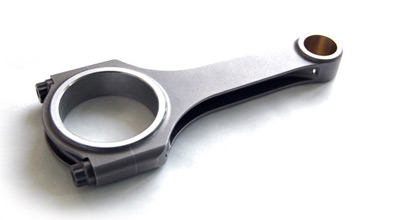
\includegraphics[width=12cm]{bielle.jpg}
\end{figure}

\end{center}
\begin{figure}[b!]
\begin{Large}
	Groupe 1\\
\end{Large}
	CHANDELLE François, 3673-13-00\\
	DISPAS David, 7189-12-00\\
	PAQUET Arnaud, 3668-13-00\\
	\\
	\newline
	\center
	
\includegraphics[width=7cm]{epl-logo.jpg}
\end{figure}
\end{titlepage}


\chapter{Réponse aux questions}

Le fonctionnement d'un moteur à explosion repose sur la conversion du mouvement alternatif du piston en rotation du vilebrequin. Cela se fait par l'intermédiaire d'une bielle. Cette pièce, répétant un cycle à raison de plusieurs milliers de fois par minute, subit des forces conséquentes. Il est donc primordial d'en faire l'analyse afin de prévoir sa forme optimale et les efforts maximaux à devoir supporter. 

\section{Mesures}

\begin{figure}	
	\center
	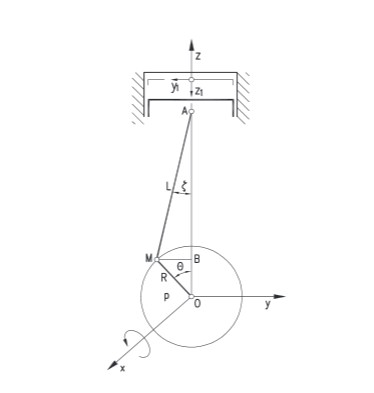
\includegraphics[scale=0.75]{Dessin.jpg}
	\caption{Piston, bielle et manivelle}
\end{figure}

Le mécanisme qui nous intéresse est un système regroupant piston, bielle et manivelle (voir figure 1.1). Notre groupe ayant reçu le vilebrequin d'une Audi A4 lors des séances de mesures, nous traiterons ici en particulier du moteur de cette voiture. De nos mesures, nous avons pu déduire la longueur R de la manivelle. Cette distance est égale à la moitié de la course du piston. Les groupes 12 et 16 nous ont donné respectivement la longueur de la bielle, L, et les longueurs des axes du piston (celui ci a en effet une forme elliptique dans notre cas). Le grand axe du piston est égal à l'alésage D des cylindres. Il est possible de trouver la cylindrée unitaire $V_c$ grâce à la formule suivante: 
$$V_c =\frac{\pi D^2 R}{2}$$

En multipliant ce volume par quatre, le nombre de cylindres, nous obtenons la cylindrée du moteur. Les valeurs réelles de R, D et $V_c$ nous ont été fournies dans un document annexe. Nous utiliserons ces données pour bénéficier d'une plus grande précision.\\

Pour finir, ne connaissant pas précisément le modèle de la voiture, nous ne pouvons qu'estimer le taux de compression, qui désigne le rapport du volume de la chambre de combustion lorsque le piston est au point minimum (en bas) sur le volume au point maximum (en haut). Une voiture dont le moteur fonctionne au diesel, a un taux de compression assez haut. Pour une audi A4, il avoisine 19.5 dans le cas d'une cylindrée égale à 1896 (comme pour la série
B5\footnote{\url{http://www.auto-data.net/en/?f=showCar&car_id=4416}}). Le résumé des mesures se trouve dans le tableau ci-dessous (voir figure 1.2).

\begin{figure}[h]
\centering
\begin{tabular}{|l|c|c|c|}
  \hline
  Longueur mesurée & Abréviation & Mesure & Distance réelle\\
  \hline
  Grand axe du piston & D & $79.4mm$ & $79.5mm$ \\
  Rayon de manivelle & R & $47mm$ & $47.75mm$\\
  Longueur de la bielle & L & $199.5mm$ & (non donné)\\
  Cylindrée unitaire & $V_c$  & $465cc$ & $474cc$\\
  Taux de compression & $\tau$ & / & $19.5$\\
  \hline
\end{tabular}
\caption{Les différentes mesures}
\end{figure}

\section{Evolution de la pression dans le cylindre}

Nous pouvons à présent analyser l'évolution de la pression dans le cylindre lors des différentes phases du moteur. Il est judicieux d'utiliser l'angle du vilebrequin $\theta$ comme variable de la fonction de pression, qui sera alors périodique de période 4$\pi$ (deux tours de vilebrequin). En partant de l'équation bien connue du premier principe de la thermodynamique nous pouvons la diviser par la différentielle de l'angle du vilebrequin, d$\theta$, et arriver sous forme simplifiée à
$$\frac{dp}{d\theta}=-\gamma\frac{p}{V}\frac{dV}{d\theta}+(\gamma - 1) \frac{1}{V}\frac{dQ}{d\theta}$$
Nous avons choisi d'utiliser une méthode de Runge Kutta d'ordre 2 pour intégrer numériquement cette équation. Cela ne se révèle utile que pour la phase de combustion, la seule où il y a un apport de chaleur non négligeable. Celui-ci est égal à $1650[kJ/kg] * V_{max} * \rho_{air}$. Les autres transformations sont considérées adiabatiques et la pression est trouvée simplement en considérant $PV^{\gamma}$ constant. L'échappement se fait avec un terme de relaxation $\frac{dp}{d\theta}=-k(p-p_atm)$ où $k=2,5$ pour que la pression retombe à 1 bar après une rotation du vilebrequin d'approximativement 30\degre.

\begin{figure}[H]
	\center
	\includegraphics[scale=0.75]{pression.jpg}
	\caption{Pression lors d'un cycle}
\end{figure}

\section{Efforts sur la bielle}

Le bilan des efforts sur la tête et le pied de bielle se mesure avec les deux formules ci-dessous. 

\begin{center}
$F_{pied} = \frac{\pi D^2}{4}p(\theta) -  m_{piston}R\omega^2 \cos(\theta)  $ \\
\end{center}
\begin{center}
$F_{tete} = -\frac{\pi D^2}{4}p(\theta) +  (m_{piston}+m_{bielle})R\omega^2 \cos(\theta)$ 
\end{center}

Voici les graphes représentant les efforts sur la bielle en fonction de l'angle du vilbrequin, à deux vitesses angulaires précises ($2500rpm$ et $4000rpm$):

\begin{figure}[H]
\center
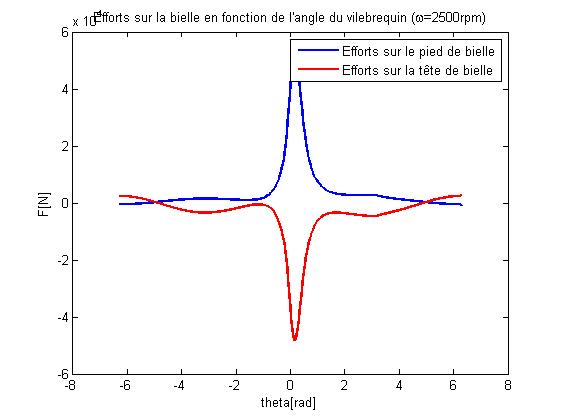
\includegraphics[scale=0.7]{effort_2500rpm.jpg}
\caption{Efforts lors d'un cycle, $\omega=2500rpm$}
\end{figure}

\begin{figure}[H]
\center
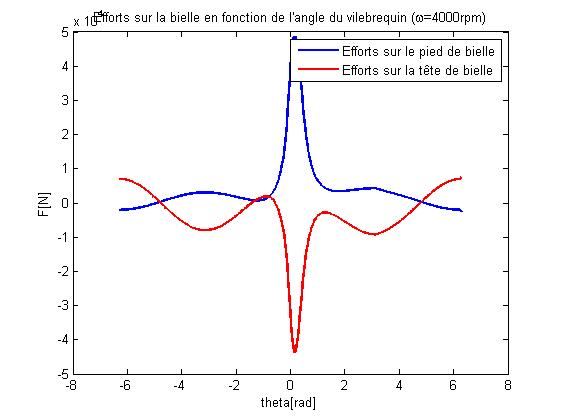
\includegraphics[scale=0.7]{effort_4000rpm.jpg}
\caption{Efforts lors d'un cycle, $\omega=4000rpm$}
\end{figure}

Les efforts maximaux et minimaux, qui s'exercent sur la bielle à ses deux extréités (pied et tête) dans le cas d'une vitesse normale de $2500rpm$, sont repris dans le tableau ci-dessous: \\

\begin{center}
\begin{tabular}{|c||c|c|}
\hline 
\ & Forces maximales [kN] & Forces minimales [kN] \\ 
\hline 
Pied de la bielle & 50.225 & -0.995 \\ 
\hline 
Tête de la bielle & 2.931 & -48.313 \\ 
\hline 
\end{tabular} \\
\end{center}

Les efforts maximaux et minimaux, qui s'exercent sur la bielle à ses deux extréités (pied et tête) dans le cas d'une vitesse élevée de $4000rpm$, sont repris dans le tableau ci-dessous: \\

\begin{center}
\begin{tabular}{|c||c|c|}
\hline 
\ & Forces maximales [kN] & Forces minimales [kN] \\ 
\hline 
Pied de la bielle & 48.692 & -2.547 \\ 
\hline 
Tête de la bielle &  7.503 & -43.798 \\ 
\hline 
\end{tabular} \\
\end{center}

\section{Justification de la forme de la bielle}

Tout d'abord, deux types de flambage sont possibles : flambage longitudinal et flambage transversal. Dans le cas de la bielle, le flambage transversal apparait plus facilement que le flambage longitudinal (à vérifier). Pour le corps de la bielle, il faut trouver le juste compromis entre masse et résistance : Plus la section du corps de la bielle est large, plus elle sera résistante mais plus lourde aussi. La configuration en I de la bielle permet une résistance élevée au flambage tout en conservant une masse moins importante. Grâce à la formule d'Euler : $F_{crit}$ = $\frac{\pi^2EI}{(l_k)^2}$ où E est le module de Young, I le moment quadratique de la bielle et $l_k$ est la longueur de flambage de la barre, on peut comparer la force critique d'une poutre profilée en I et celle d'une poutre de section carrée pour une section d'aire équivalente. Le module de Young étant propre au matériau et $l_k$ le même pour les deux bielles, le seul moyen de maximiser la force à partir de laquelle la bielle flambera est de trouver la forme pour laquelle le moment quadratique [unité: $m^4$] est maximal. Voici la formule du moment quadratique d'une poutre profilée I : $\frac{t}{12}h^3\frac{1+3s}{h}$ où t est la largeur de l'âme, s, la largeur de la semelle et h, la hauteur de l'âme.

\section{Dimensionnement de la bielle}

Le risque de flambage sera accru lorsque la bielle est longue et de faible section.
On voit sur ce graphe (insérer graphe page 24) qu'à $5400rpm$ la bielle subit une force maximale lors du cycle de $10.000 N$.
En admettant que la bielle ait été obtenue par moulage, son module de Young vaut $170.000 MPa$, 

\chapter{Annexe}

Code Matlab ?

\end{document}